% ====================== Robotics Control Full Lecture ======================
\documentclass{beamer}
\usetheme{Madrid}
\usecolortheme{dolphin}
\usepackage{amsmath,amssymb,mathtools}
\usepackage{tikz}
\usepackage{graphicx}
\usepackage{tcolorbox}
\tcbuselibrary{theorems}
\usetikzlibrary{arrows.meta, positioning}

% Color-coded notes and theorems
\definecolor{noteBg}{RGB}{250,240,230}
\definecolor{noteFrame}{RGB}{200,120,40}
\newtcolorbox{noteBox}{colback=noteBg,colframe=noteFrame,arc=4pt,boxrule=0.8pt}
\newtcolorbox{theoremBox}{colback=white!95!blue!5,colframe=blue!60!black,fonttitle=\bfseries,arc=4pt,boxrule=0.8pt}

% Title
\title{Robotics Control -- Detailed Lecture}
\subtitle{Based on Spong, Hutchinson \& Vidyasagar (Ch.8-9)}
\author{}
\date{}

\begin{document}
	
	% ====================== Title Page ======================
	\begin{frame}
		\titlepage
	\end{frame}
	
	\begin{frame}{Outline}
		\tableofcontents
	\end{frame}
	
	% ====================== Dynamics ======================
	\section{Robot Dynamics}
	
	\begin{frame}{Euler--Lagrange Dynamics}
		Robot manipulator dynamics:
		\[
		M(q)\ddot{q} + C(q,\dot{q})\dot{q} + g(q) = \tau
		\]
		
		\begin{noteBox}
			$M(q)$: inertia matrix, $C(q,\dot q)$: Coriolis/centrifugal, $g(q)$: gravity vector. Derived from Lagrangian $L=K-P$.
		\end{noteBox}
		$M(q)$ symmetric positive definite. $\dot M - 2C$ skew-symmetric. Implies:
		\[
		\dot q^T (M\ddot q + C\dot q) = \frac{d}{dt} \left(\frac12 \dot q^T M \dot q\right)
		\]
		
		This property is central for Lyapunov stability proofs.
	\end{frame}
	
	\begin{frame}{1-DOF Pendulum -- Dynamics Derivation}
		Kinetic energy:
		\[
		K = \frac12 m (l\dot q)^2 = \frac12 m l^2 \dot q^2
		\]
		
		Potential energy:
		\[
		P = m g l (1 - \cos q)
		\]
		
		Lagrangian:
		\[
		L = K - P
		\]
		
		Euler-Lagrange:
		\[
		\frac{d}{dt} \frac{\partial L}{\partial \dot q} - \frac{\partial L}{\partial q} = \tau
		\]
		
		Step by step:
		\[
		\frac{\partial L}{\partial \dot q} = m l^2 \dot q, \quad 
		\frac{d}{dt} \frac{\partial L}{\partial \dot q} = m l^2 \ddot q
		\]
		\[
		\frac{\partial L}{\partial q} = m g l \sin q
		\]
		
		Dynamics:
		\[
		m l^2 \ddot q + m g l \sin q = \tau
		\]
	\end{frame}
	
	\begin{frame}{1-DOF Pendulum}
		\centering
		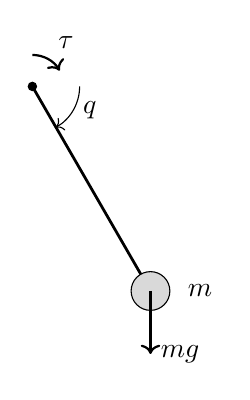
\begin{tikzpicture}[scale=1]
			\coordinate (O) at (0,0);
			\draw[fill=black] (O) circle (1.5pt);
			\draw[line width=1pt] (O) -- ++(-60:3) coordinate (B);
			\draw[fill=gray!30] (B) circle (7pt) node[right=10pt]{$m$};
			\draw[->] (0.6,0) arc (0:-60:0.6) node[midway,right]{$q$};
			\draw[->,thick] (B) -- ++(0,-0.8) node[right]{$mg$};
			\draw[->,thick] (0,0.4) arc (90:30:0.4) node[midway,above right]{$\tau$};
		\end{tikzpicture}
		
			
		
	\end{frame}
	
	\begin{frame}{Control of Manipulators}
			\begin{itemize}
			\item The control problem for robot manipulators is to determine the time
			history of joint inputs required to cause the end eector to execute a commanded
			motion.
			\item There are many control techniques and methodologies that can be applied
			to the control of manipulators. The particular control method used
			can have a signicant impact on the performance of the manipulator and
			consequently on the range of its possible applications.
			\item The mechanical design of the manipulator itself will influence 			the type of control scheme needed, eg: a robot actuated by permanent magnet DC motors
			with gear reduction will have different issues compared to a direct-drive robot using high-torque motors with no gear reduction. 
		\end{itemize}
	\end{frame}
	
	% ====================== Classical Control ======================
	\section{Classical Control}
	\begin{frame}{Independant Joint Control}
		\textbf{Definition}
		\begin{itemize}
			\item Independent joint control is a simple type of control strategy. In this type of control each axis of the manipulator
			is controlled as a single-input/single-output (SISO) system.
		\end{itemize}
	
	\end{frame}
	\begin{frame}{PD + Gravity Compensation}
		\textbf{Control law:}
		\[
		\tau = K_p (q_d - q) + K_d (\dot q_d - \dot q) + g(q)
		\]
		
		\begin{noteBox}
			Cancels gravity, applies PD control on tracking error.
		\end{noteBox}
	\end{frame}
	
	\begin{frame}{Example: Pendulum Regulation}
		Desired: $q_d=0$, $\dot q_d=0$. Controller:
		\[
		\tau = -K_p q - K_d \dot q + m g l \sin q
		\]
		
		Linearize $\sin q \approx q$:
		\[
		m l^2 \ddot q + K_d \dot q + (K_p - m g l) q = 0
		\]
		
		Choose $K_p > m g l$ for stability.
	\end{frame}
	
	% ====================== Computed Torque ======================
	\section{Computed Torque / Inverse Dynamics}
	
	\begin{frame}{Computed Torque Controller}
		Linearizing error dynamics:
		\[
		v = \ddot q_d + K_d (\dot q_d - \dot q) + K_p (q_d - q)
		\]
		
		Control law:
		\[
		\tau = M(q) v + C(q,\dot q)\dot q + g(q)
		\]
		
		Error dynamics:
		\[
		\ddot e + K_d \dot e + K_p e = 0
		\]
	\end{frame}
	
	\begin{frame}{2-DOF Planar Arm}
		\centering
		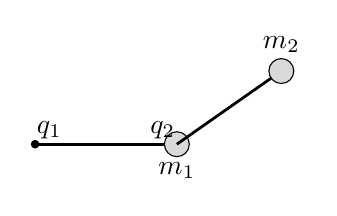
\begin{tikzpicture}[scale=0.9]
			\coordinate (O) at (0,0);
			\draw[fill=black] (O) circle (1.5pt);
			\draw[line width=1pt] (O) -- (2,0) coordinate (A);
			\draw[fill=gray!30] (A) circle (5pt) node[below=3pt]{$m_1$};
			\draw[line width=1pt] (A) -- ++(35:1.8) coordinate (B);
			\draw[fill=gray!30] (B) circle (5pt) node[above=3pt]{$m_2$};
			\draw (0,0) ++(0.2,0.2) node{$q_1$};
			\draw (2,0) ++(-0.2,0.2) node{$q_2$};
		\end{tikzpicture}
	\end{frame}
	
	% ====================== Adaptive Control ======================
	\section{Adaptive Control}
	
	\begin{frame}{Adaptive Control: Linear in Parameters}
		\[
		M\ddot q + C\dot q + g = Y(q,\dot q,\ddot q) \theta
		\]
		
		\begin{theoremBox}[title=Adaptive Law]
			\[
			\dot{\hat\theta} = -\Gamma Y^T s, \quad s = \dot e + \Lambda e
			\]
			
			Then $s \to 0$ and tracking achieved.
		\end{theoremBox}
	\end{frame}
	
	\begin{frame}{1-DOF Adaptive Example}
		Reference acceleration:
		\[
		\ddot q_r = \ddot q_d + K_d (\dot q_d - \dot q) + K_p (q_d - q)
		\]
		
		Adaptive law updates estimates of $ml^2$ and $mgl$ online.
	\end{frame}
	
	% ====================== Sliding Mode Control ======================
	\section{Sliding Mode Control}
	
	\begin{frame}{Sliding Mode Control}
		Sliding variable:
		\[
		s = \dot e + \lambda e
		\]
		
		Controller with boundary layer:
		\[
		\tau = \tau_{eq} - K \, \mathrm{sat}(s/\phi)
		\]
		
		\begin{noteBox}
			Reduces chattering while enforcing sliding surface.
		\end{noteBox}
	\end{frame}
	
	% ====================== Disturbance Observers ======================
	\section{Disturbance Observers}
	
	\begin{frame}{Disturbance Observer Block Diagram}
		\centering
		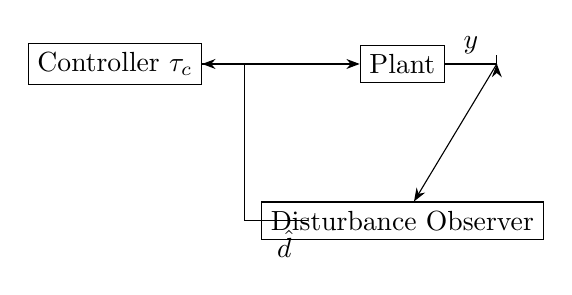
\begin{tikzpicture}[auto,node distance=2cm,>=Stealth]
			\node[draw,rectangle] (controller) {Controller $\tau_c$};
			\node[draw,rectangle,right=2cm of controller] (plant) {Plant};
			\node[draw,rectangle,below=1.5cm of plant] (observer) {Disturbance Observer};
			\draw[->] (controller) -- (plant);
			\draw[->] (plant) -- ++(1.2,0) node[midway,above]{$y$} -- ++(0,0) coordinate (yout);
			\draw[->] (yout) -- (observer);
			\draw[->] (observer) -- ++(-1.2,0) node[midway,below]{$\hat d$} -- ++(-0.8,0) |- (controller);
		\end{tikzpicture}
	\end{frame}
	
	% ====================== Exercises ======================
	\section{Exercises and Solutions}
	
	\begin{frame}{Exercise 1}
		1-DOF pendulum: derive Euler-Lagrange dynamics and identify $M, C, g$.
	\end{frame}
	
	\begin{frame}{Solution 1}
		Kinetic energy:
		\[
		K = \tfrac12 m l^2 \dot q^2, \quad
		P = m g l (1 - \cos q)
		\]
		
		Euler-Lagrange:
		\[
		\frac{d}{dt}(m l^2 \dot q) + m g l \sin q = \tau
		\]
		
		Therefore:
		\[
		M = m l^2, \quad C = 0, \quad g(q) = m g l \sin q
		\]
	\end{frame}
	
	\begin{frame}{References}
		\begin{itemize}
			\item M. W. Spong, S. Hutchinson, M. Vidyasagar, ``Robot Modeling and Control''
			\item Lecture notes and examples adapted for teaching
		\end{itemize}
	\end{frame}
	
\end{document}
